\documentclass[12pt,compress]{beamer}
%\documentclass[handout,t]{beamer}

\batchmode
% \usepackage{pgfpages}
% \pgfpagesuselayout{4 on 1}[letterpaper,landscape,border shrink=5mm]

\usepackage{amsmath,amssymb,enumerate,epsfig,bbm,calc,color,ifthen,capt-of,caption}

\usepackage[all,pdf]{xy}

% add page number
\expandafter\def\expandafter\insertshorttitle\expandafter{%
	\insertshorttitle\hfill%
	\insertframenumber\,/\,\inserttotalframenumber}

\usetheme{Berlin}
\usecolortheme{umji}

\title{Gas-Liq-Solids \\ Three-laws-Thermo}
\author{Haotian Fu}
\institute{University of Michigan--Shanghai Jiao Tong University Joint Institute}
\date{\today}
\pgfdeclareimage[height=0.5cm]{umji-logo}{umji.pdf}

\logo{\pgfuseimage{umji-logo}\hspace*{0.5cm}}

\AtBeginSection[]
{
\begin{frame}<beamer>
    \frametitle{Outline}
    \tableofcontents[currentsection]
\end{frame}
}
\beamerdefaultoverlayspecification{<+->}

% -----------------------------------------------------------------------------
\begin{document}

% -----------------------------------------------------------------------------

\lecture{RC_\#}

\frame{\titlepage}

\section[Outline]{}
\begin{frame}{Outline}
	\tableofcontents
\end{frame}

% -----------------------------------------------------------------------------

\section{States of Matter}
\subsection{Gas, Liquid, and Solid}
\begin{frame}{General Notice}
	\begin{itemize}
		\item unit: Kelvin(K) \& J$\cdot$K$^{-1}\cdot$mol$^{-1}$
		\item status: SATP \& STP
		\item formula transformation: molartity \& density
	\end{itemize}
\end{frame}
\begin{frame}{Gas}
	\begin{block}{$pV=nRT$}
		How to understand ideal gas equation?
		\begin{itemize}
			\item empirical law?
		\end{itemize}
	\end{block}
	\begin{block}{$v_{\rm rms}=\sqrt{3RT/M}$}
		Why do we study kinetic molecular theory?
		\begin{itemize}
			\item Graham’s law of effusion?
		\end{itemize}
	\end{block}
\end{frame}
\begin{frame}{Understanding from A New Point of View}
	Here we will discuss the \textbf{ideal gas equation} from a new point of view,
	\textit{i.e.}, \textbf{kinetic molecular theory}(KMT).
\end{frame}
\begin{frame}{Understanding from A New Point of View}
	First we should get aware of the \textbf{prerequisite} of KMT. \\
	\pause
	Recall what has been taught in lectures.
	\begin{figure}[!htbp]
		\centering
		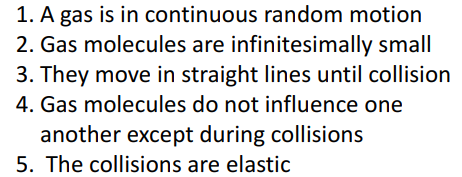
\includegraphics[width=0.8\textwidth]{KMT_slide.png}
		\caption*{\footnotesize{Prerequisites of KMT shown in slides\footnote{\tiny{Sun, Ting, \textit{CHEM2100J-FA21-Ch5-6}, pp. 35.}}}}
	\end{figure}
\end{frame}
\begin{frame}{Understanding from A New Point of View}
	Now we conclude
	\begin{itemize}
		\item \textcolor{gray}{A gas is in continuous random motion} and
		      evenly distributed throughout the container. Irregular molecular
		      movement does not do work.
		\item Substances of the same chemical properties have the same particle size,
		      shape and functions.
		\item \textcolor{gray}{Gas molecules are infinitesimally small and they move in straight
			      lines until collision.}
		\item \textcolor{gray}{Gas molecules do not influence one another except
			      during collisions.}
		\item \textcolor{gray}{The collisions are elastic.}
	\end{itemize}
\end{frame}
\begin{frame}{Understanding from A New Point of View}
	\textbf{Example}
	\par For a model satisfying KMT, suppose there exists $N$ gas molecules in a cubic box with length $L$. Each molecule has the mass of $m$,
	and the speed of $u$.
	\begin{figure}[!htbp]
		\centering
		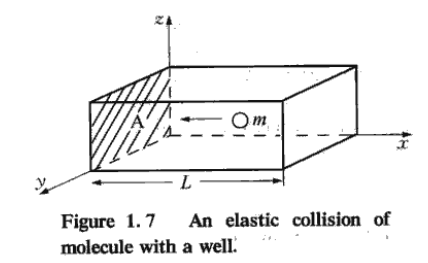
\includegraphics[width=0.5\textwidth]{KMT.png}
	\end{figure}
\end{frame}
\begin{frame}{Understanding from A New Point of View}
	(1) Calculate the average kinetic energy of each molecule $\bar{E_k}$.
	(2) If the relationship between average molecule and the temperature is
	\begin{equation*}
		\bar{E_k} = \frac{3}{2}kT
	\end{equation*}
	where $k$ denotes the Boltzmann constant and satisfies $k = \frac{R}{N_A}$,
	\par what familar formula will derived?
\end{frame}

\begin{frame}{Liquid}
	\begin{itemize}
		\item viscosity
		\item surface tension
		      \begin{figure}[!htbp]
			      \centering
			      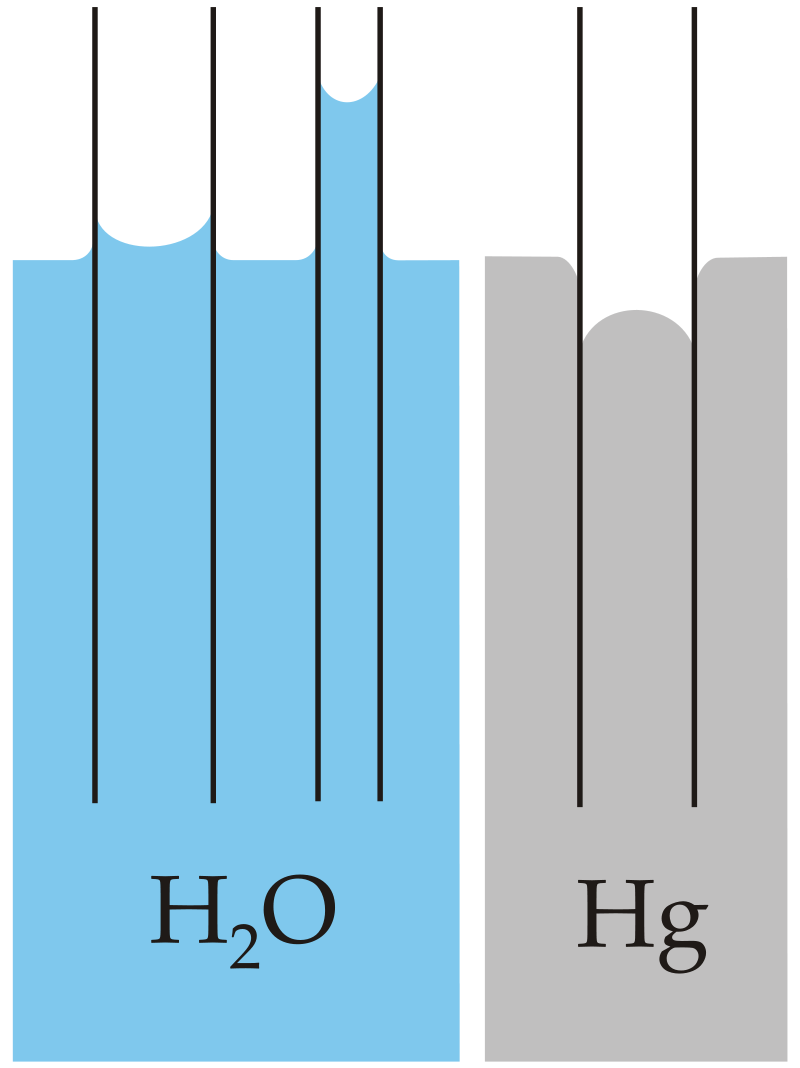
\includegraphics[width=0.3\textwidth]{Capillarity.png}
		      \end{figure}
	\end{itemize}
\end{frame}

\begin{frame}{Solid}
	\begin{itemize}
		\item crystalline \& amorphous
		\item Molecular Solids \& Network Solids \& Metallic Solids
	\end{itemize}
\end{frame}

\begin{frame}{Closed-Packed Structures}
	\begin{figure}[!htbp]
		\begin{minipage}{14cm}
			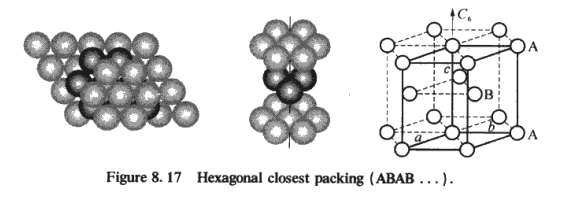
\includegraphics[width=0.4\textwidth]{hcp.png}
			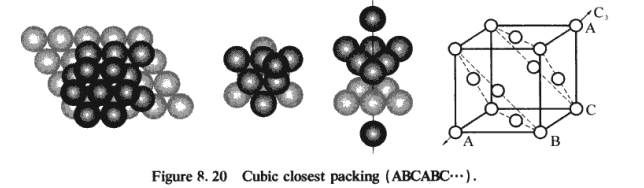
\includegraphics[width=0.4\textwidth]{ccp.png}
		\end{minipage}
	\end{figure}
	\begin{block}{How to understand packed structures?}
		What is packed structures/closed-packed structures? \\ 
		What does $A,B,C$ mean? \\ 
		How to calculate the occupied rate?
	\end{block}
\end{frame}

\subsection{Intermolecular Forces}
\begin{frame}{Intermolecular Forces}
	\textcolor{red}{The key to understanding intermolecular forces is to understand the way to form chemical bonds.}
	\par Several ways to consider
	\begin{itemize}
		\item polarity
		\item spacial geometries
		\item chemical elements
	\end{itemize}
\end{frame}
\begin{frame}{Intermolecular Forces}
	\begin{table}[!htbp]
		\begin{tabular}{|c|c|c|c|}
			\hline
			                 & Ion-Ion       & Ion-Dipole      & Dipole-Dipole   \\ \hline
			$E_p$ dependence & $\frac{1}{r}$ & $\frac{1}{r^2}$ & $\frac{1}{r^3}$ \\ \hline
		\end{tabular}
	\end{table}
	\begin{table}[!htbp]
		\begin{tabular}{|c|c|c|c|}
			\hline
			                 & \begin{tabular}[c]{@{}l@{}}Dipole-Dipole\\ (induced)\end{tabular} & London          & \begin{tabular}[c]{@{}l@{}}Hydrogen\\ Bonding\end{tabular} \\ \hline
			$E_p$ dependence & $\frac{1}{r^6}$            & $\frac{1}{r^6}$ & $\slash$                   \\ \hline
		\end{tabular}
	\end{table}

	\textbf{Remarks:} In daily life, Total Price = Unit Price $\times$ Amount. So is chemistry.
\end{frame}
\begin{frame}{Hydrogen Bonding}
	\begin{figure}
		\centering 
		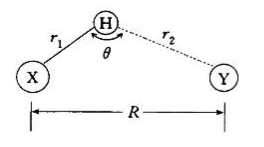
\includegraphics[width=0.4\textwidth]{hydrogen_bond.png}
	\end{figure}
	\begin{itemize}
		\item Tend to be formed and can be formed easily.
		\item Both intermolecular or intramolecular.
		\item Depends on the geometry, the environment, and the nature of the specific donor and acceptor atoms, varying between a large range.
	\end{itemize}
\end{frame}
\begin{frame}{Hydrogen Bonding}
	Examples of hydrogen bond
	\begin{itemize}
		\item The density of water and ice.
		\item The acidity of HF.
		\item Alcohol solution
	\end{itemize}
\end{frame}

% -----------------------------------------------------------------------------

\section{Thermodynamics}
\subsection{Introduction}
\begin{frame}{Introduction}
	\textbf{\textcolor{red}{\LARGE The key to understanding theomodynamics is to design thermodynamic cycle.}}
\end{frame}
\begin{frame}{Key Concepts}
	\begin{itemize}
		\item system \& surrounding
		\item work \& heat \& energy \\ 
			The First Law $\Delta U = q + w$
			\begin{itemize}
				\item expansion work
				\item state function
				\item heat capacity
				\item internal energy
				\item enthalpy
				\begin{itemize}
					\item constant pressure
					\item constant volume
				\end{itemize}
				\item heating curve
			\end{itemize}
		\item Hess's Law
		\item The Born-Haber Cycle
	\end{itemize}
\end{frame}
\begin{frame}{The First Law}
	$\Delta U = q + w$
	\begin{itemize}
		\item state function
		\item sign
	\end{itemize}
\end{frame}
\begin{frame}{Expansion Work}
	\begin{equation*}
		\delta W = -pdV
	\end{equation*}
	\begin{itemize}
		\item free expansion
		\item expansion at constant pressure
		\item expansion at constant temperature
		\item reversible expansion
	\end{itemize}
\end{frame}
\begin{frame}{Heat Capacity}
	\begin{itemize}
		\item Definition: $C = \frac{q}{\Delta T}$
			\begin{itemize}
				\item specific heat capacity: $C_s = \frac{C}{m}$
				\item molar heat capacity: $C_m = \frac{C}{n}$
			\end{itemize}
	\end{itemize}

\end{frame}
\begin{frame}{Enthalpy}
	\begin{itemize}
		\item definition
		\item origin
		\item constant pressure and constant volume
		\item relationship between heat capacity
	\end{itemize}
\end{frame}

\subsection{Examples}
\begin{frame}{Expansion}
	\textbf{Example}
	\par 10 mol ideal gas expands at 300 K, with initial volume $V_1 = 25$ dm$^3$, final volume $V_2 = 100$ dm$^3$,
	experiencing the following four paths: \\ 
	(1) free expansion; \\ 
	(2) expands at final pressure when it is 100 dm$^3$; \\ 
	(3) first expands at the initial pressure until it is 50 dm$^3$, then expands at the final pressure until final state; \\ 
	(4) reversible expansion.
\end{frame}
\begin{frame}{Hess's Law}
	\textbf{Example}
	\begin{figure}
		\centering
		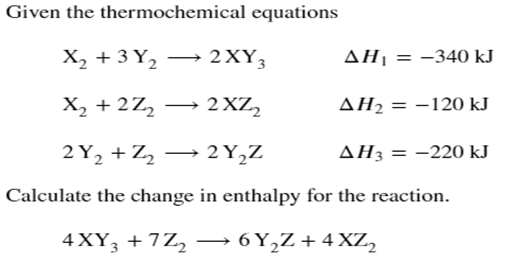
\includegraphics[width=0.8\textwidth]{hess's_law.png}
	\end{figure}
\end{frame}
\begin{frame}{The Born-Haber Cycle}
	\textbf{Example}
	\par At $p^\ominus$ and 298.15 K, mix 1 mol CH$_4$ and 4 mol O$_2$ and fire them to make them explode under
	constant pressure. Suppose this  reaction happens in an instaneous moment. Calculate the higher temperature this system
	may achieve. \\ 
	Data: \\ 
	$\Delta_{\mathrm{f}} H_{\mathrm{m}}^{\ominus}\left(\mathrm{CO}_{2}, \mathrm{~g}\right)=-393.51 \mathrm{~kJ} \cdot \mathrm{mol}^{-1}$ \\ 
	$\Delta_{\mathrm{f}} H_{\mathrm{m}}^{\ominus}\left(\mathrm{H}_{2} \mathrm{O}, \mathrm{g}\right)=-241.82 \mathrm{~kJ} \cdot \mathrm{mol}^{-1}$ \\ 
	$\Delta_{\mathrm{r}} H_{\mathrm{m}}^{\ominus}\left(\mathrm{CH}_{4}, \mathrm{~g}\right)=-74.81 \mathrm{~kJ} \cdot \mathrm{mol}^{-1}$
\end{frame}

%------------------------------------------------------------------------------

\section{Conclusions}

\subsection{As for States of Matter}
\begin{frame}{Remarks}
	\begin{itemize}
		\item You can never be too careful about \textcolor{red}{UNITS}.
		\item Relate concepts to questions properly. \textcolor{red}{Undertand the concepts}.
		\item Undertanding is always more important than just using.
	\end{itemize}
\end{frame}

\subsection{As for Thermodynamics}
\begin{frame}{Remarks}
	\begin{itemize}
		\item Process: constant pressure, constant volume, adiatic
		\item Example: vaporation, fusion, freezing, condensation, sublimation, deposition, expansion
		\item Know the concepts and design your cylce smartly.
	\end{itemize}
\end{frame}

% -----------------------------------------------------------------------------

\end{document}